\chapter{Results} \label{chapter:results}
% Setup, supercomputers etc
% Profiler
% Memory usage maybe?
% Stream performance
% Mixed precision maybe?
% Hybrid solver?
% Different block sizes!!

Following are results studying the effectiveness of the program. Three main components are studied.
First, the performance of the core spectral element method code on GPUs, with a comparison with the
same code running on CPUs is presented in Section~\ref{section:results:scaling_tests}. Then, the
performance of the adaptive mesh refinement is studied in
Section~\ref{section:results:adaptivity_performance}. Finally, dynamic load balancing is studied in
Section~\ref{section:results:load_balancing_performance}.

\section{Platforms} \label{section:results:platforms}
This program aims to perform large scale computations, and as such targets HPC platforms. The
program has been designed to scale to multiple parallel level, the highest being splitting the
workload between several HPC nodes, each having multiple CPUs and GPUs. To test this use case,
most of the following tests were run on clusters graciously offered by Compute
Canada\footnote{https://www.computecanada.ca/}. Two such clusters were used for our experiments,
Béluga and Narval.

\subsection{Béluga} \label{section:results:platforms:beluga}
Béluga is a heterogeneous cluster suitable for a variety of purposes, from traditional CPU computing
to massively parallel GPU computing. It is located at the École de technologie supérieure in
Montréal. Beluga is made up of 977 compute nodes of different types, totaling 39,120 CPU cores and
696 GPUs. For our testing, we use Béluga's GPU nodes. Each one of the 172 GPU nodes contains 40 CPU
cores and 186 GB of memory across two Intel Gold 6148 CPUs, and four NVidia V100 SXM2 GPUs with 16
GB of memory each. One such node totals about 2 TFlops of CPU computing power, and 13 TFlops of GPU
computing power. The nodes are connected by Infiniband HDR (100 Gb/s) interconnections.

\subsection{Narval} \label{section:results:platforms:narval}
Narval is a heterogeneous cluster suitable for a variety of purposes, from traditional CPU computing
to massively parallel GPU computing and artificial intelligence workloads. It is located at the
École de technologie supérieure in Montréal. Beluga is made up of 1301 compute nodes of different
types, totaling 80,720 CPU cores and 636 GPUs. For our testing, we use Narval's GPU nodes. Each one
of the 159 GPU nodes contains 48 CPU cores and 498 GB of memory across two AMD Milan 7413 CPUs, and
four NVidia A100 GPUs with 40 GB of memory each. One such node totals about 2.2 TFlops of CPU
computing power, and 38.8 TFlops of GPU computing power. The nodes are connected by Infiniband EDR
(100 Gb/s) interconnections.

\subsection{Consumer hardware} \label{section:results:platforms:consumer}
Some smaller scale tests or tests that didn't involve performance were run on consumer hardware.
This is important, as it may not always be possible to access HPC systems when flow simulations have
to be performed. The program should also have reasonable performance on regular systems. The system
used in these cases is a single computer containing 16 CPU cores and 128 GB of memory across two
Intel E5-2650 V2 CPUs, and one NVidia GTX 1070 GPU with 8 GB of memory. This is an interesting
comparison, as consumer GPUs are not geared towards high precision compute loads. GPUs found in HPC
systems typically have a 1:2 ratio between their double precision and single precision performance,
whereas consumer GPUs usually have 1:32 ratio. This means that computations using double precision
floating point numbers will execute at one sixteenth of the speed of compute-oriented GPUS, all
other factors being equal.

\section{Test case} \label{section:results:test_case}
% new case

\begin{figure}[H]
	\centering
	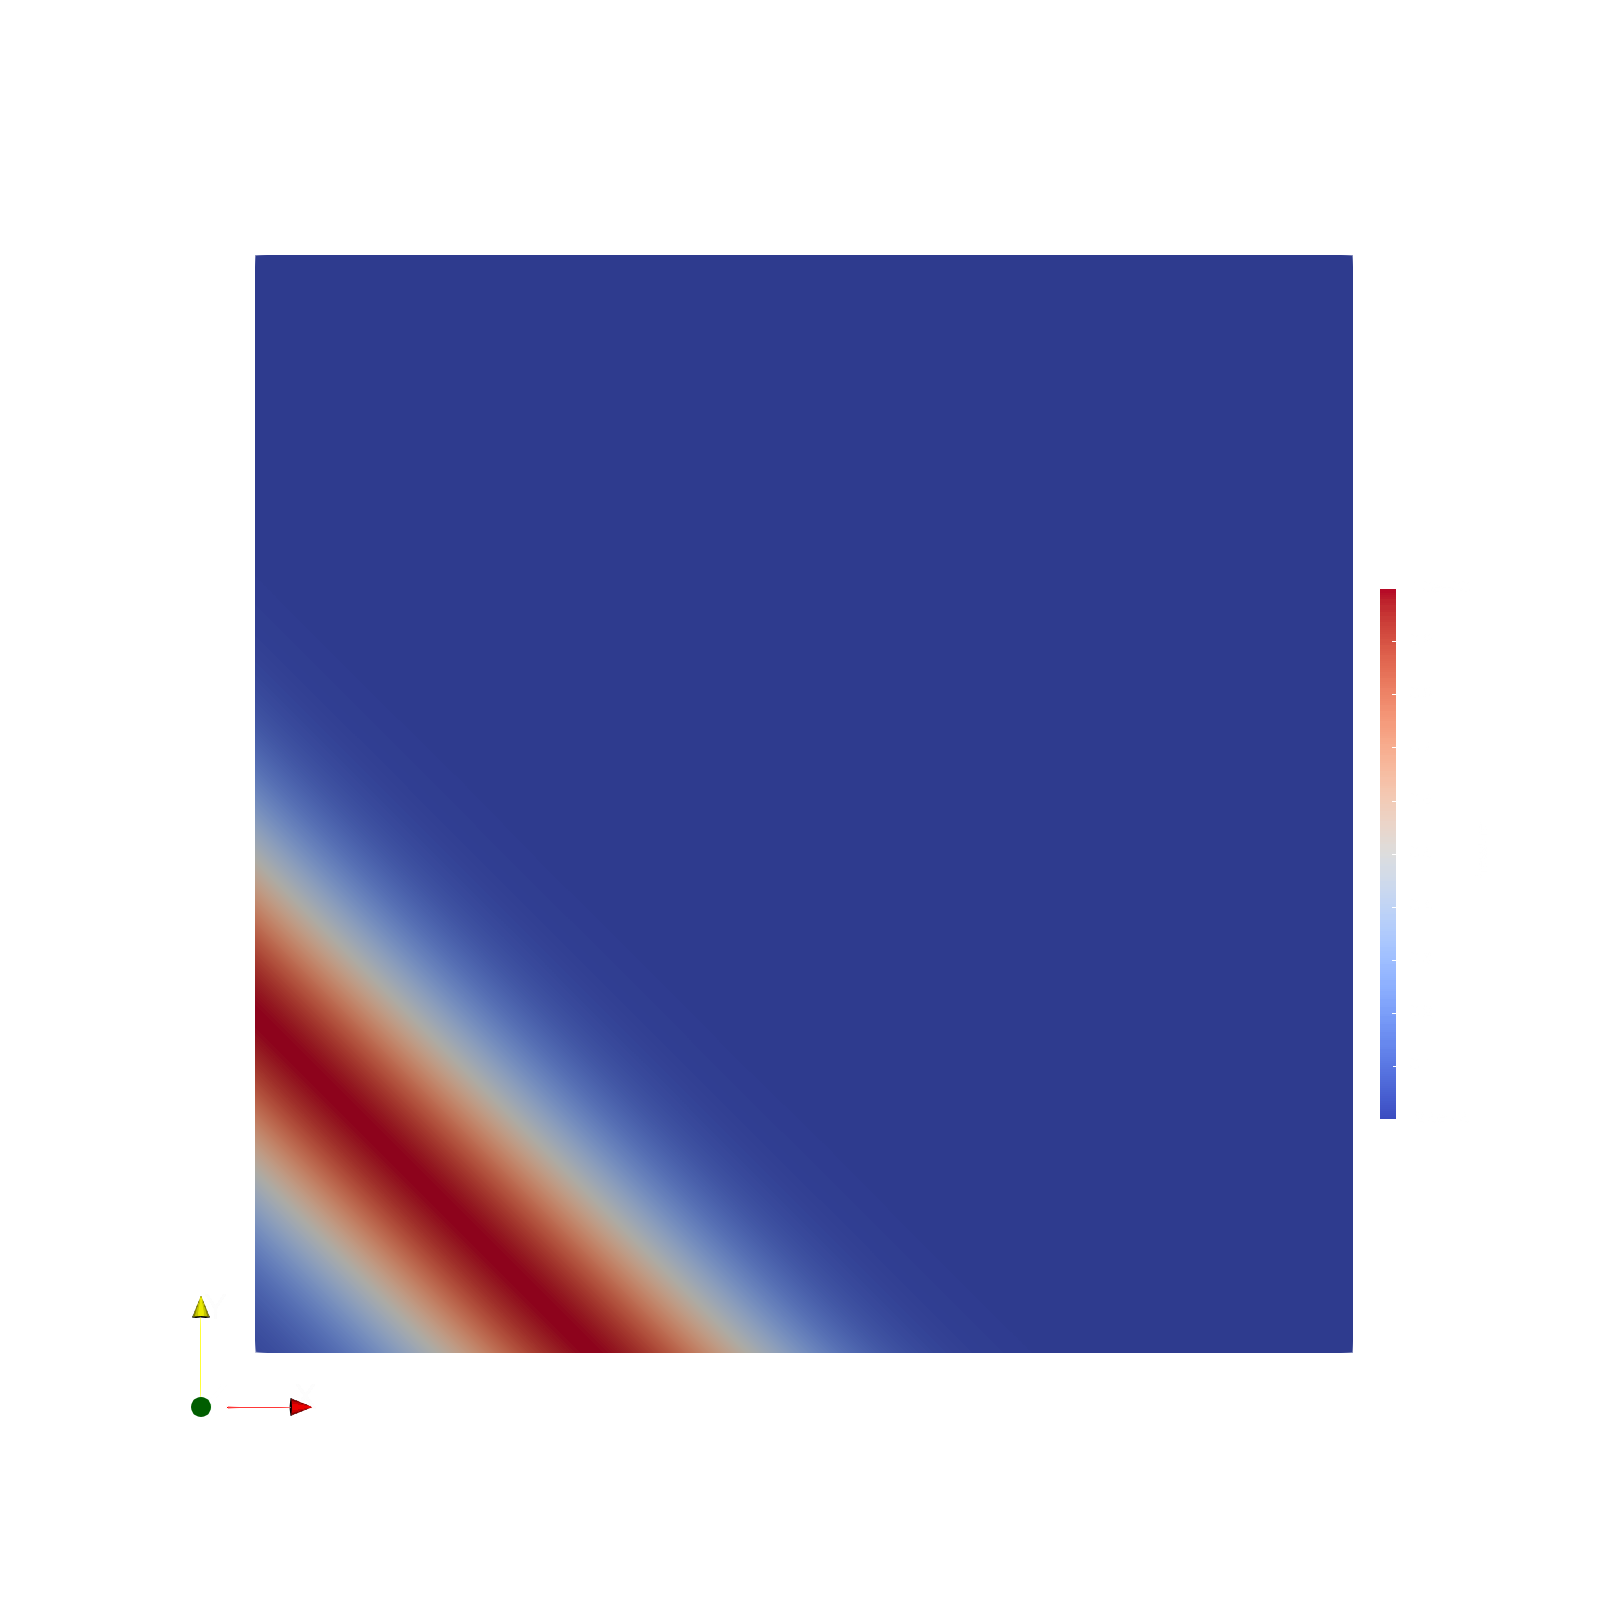
\includegraphics[width=0.6\textwidth]{Chapter_results/media/problem_1}
	\caption{Test case: A wave travels through a square domain at a 45° angle.}
	\label{fig:problem}
\end{figure}

\section{Scaling tests} \label{section:results:scaling_tests}
% Scaling tests (strong and weak), N tests
% CPU vs GPU
% GPU loading

\subsection{Strong scaling} \label{section:results:scaling_tests:strong}

\begin{figure}[H]
	\centering
	\includesvg[width=0.6\textwidth]{Chapter_results/media/strong_scaling_N4_K65536_W32}
	\caption{Weak scaling: The problem size increases with the number of workers. N = 4, K = 65536, W = 32}
	\label{fig:strong_scaling_N4_W32}
\end{figure}

\begin{figure}[H]
	\centering
	\includesvg[width=0.6\textwidth]{Chapter_results/media/strong_scaling_N6_K65536_W32}
	\caption{Weak scaling: The problem size increases with the number of workers. N = 6, K = 65536, W = 32}
	\label{fig:strong_scaling_N6_W32}
\end{figure}

\begin{figure}[H]
	\centering
	\includesvg[width=0.6\textwidth]{Chapter_results/media/strong_scaling_N6_K65536_W64}
	\caption{Weak scaling: The problem size increases with the number of workers. N = 6, K = 65536, W = 64}
	\label{fig:strong_scaling_N6_W64}
\end{figure}

\begin{figure}[H]
	\centering
	\includesvg[width=0.6\textwidth]{Chapter_results/media/strong_scaling_N6_K65536_W128}
	\caption{Weak scaling: The problem size increases with the number of workers. N = 6, K = 65536, W = 128}
	\label{fig:strong_scaling_N6_W128}
\end{figure}

\subsection{Weak scaling} \label{section:results:scaling_tests:weak}

\begin{figure}[H]
	\centering
	\includesvg[width=0.6\textwidth]{Chapter_results/media/weak_scaling_N4_K4096_W32}
	\caption{Weak scaling: The problem size increases with the number of workers. N = 4, K = 4096/worker, W = 32}
	\label{fig:weak_scaling}
\end{figure}

\section{Adaptive mesh refinement performance} \label{section:results:adaptivity_performance}
% Error adaptive vs non-adaptive, time to run
% Error at same runtime

\begin{figure}[H]
	\centering
	\includesvg[width=0.6\textwidth]{Chapter_results/media/adaptivity_N4_K16_C5}
	\caption{Adaptivity efficiency: Simulation time and analytical error with adaptivity and increasing pre-processing steps. N = 4, K = 16, adaptivity interval = 5}
	\label{fig:adaptivity_efficiency_C5}
\end{figure}

\begin{figure}[H]
	\centering
	\includesvg[width=0.6\textwidth]{Chapter_results/media/adaptivity_N4_K16_C20}
	\caption{Adaptivity efficiency: Simulation time and analytical error with adaptivity and increasing pre-processing steps. N = 4, K = 16, adaptivity interval = 20}
	\label{fig:adaptivity_efficiency_C20}
\end{figure}

\begin{figure}[H]
	\centering
	\includesvg[width=0.6\textwidth]{Chapter_results/media/adaptivity_N4_K16_C100}
	\caption{Adaptivity efficiency: Simulation time and analytical error with adaptivity and increasing pre-processing steps. N = 4, K = 16, adaptivity interval = 100}
	\label{fig:adaptivity_efficiency_C100}
\end{figure}

\begin{figure}[H]
	\centering
	\includesvg[width=0.6\textwidth]{Chapter_results/media/adaptivity_N4_K16_C500}
	\caption{Adaptivity efficiency: Simulation time and analytical error with adaptivity and increasing pre-processing steps. N = 4, K = 16, adaptivity interval = 500}
	\label{fig:adaptivity_efficiency_C500}
\end{figure}

\section{Dynamic load balancing performance} \label{section:results:load_balancing_performance}
% Runtime adaptive with and without load balancing

\begin{figure}[H]
	\centering
	\subfloat[Pressure]
	{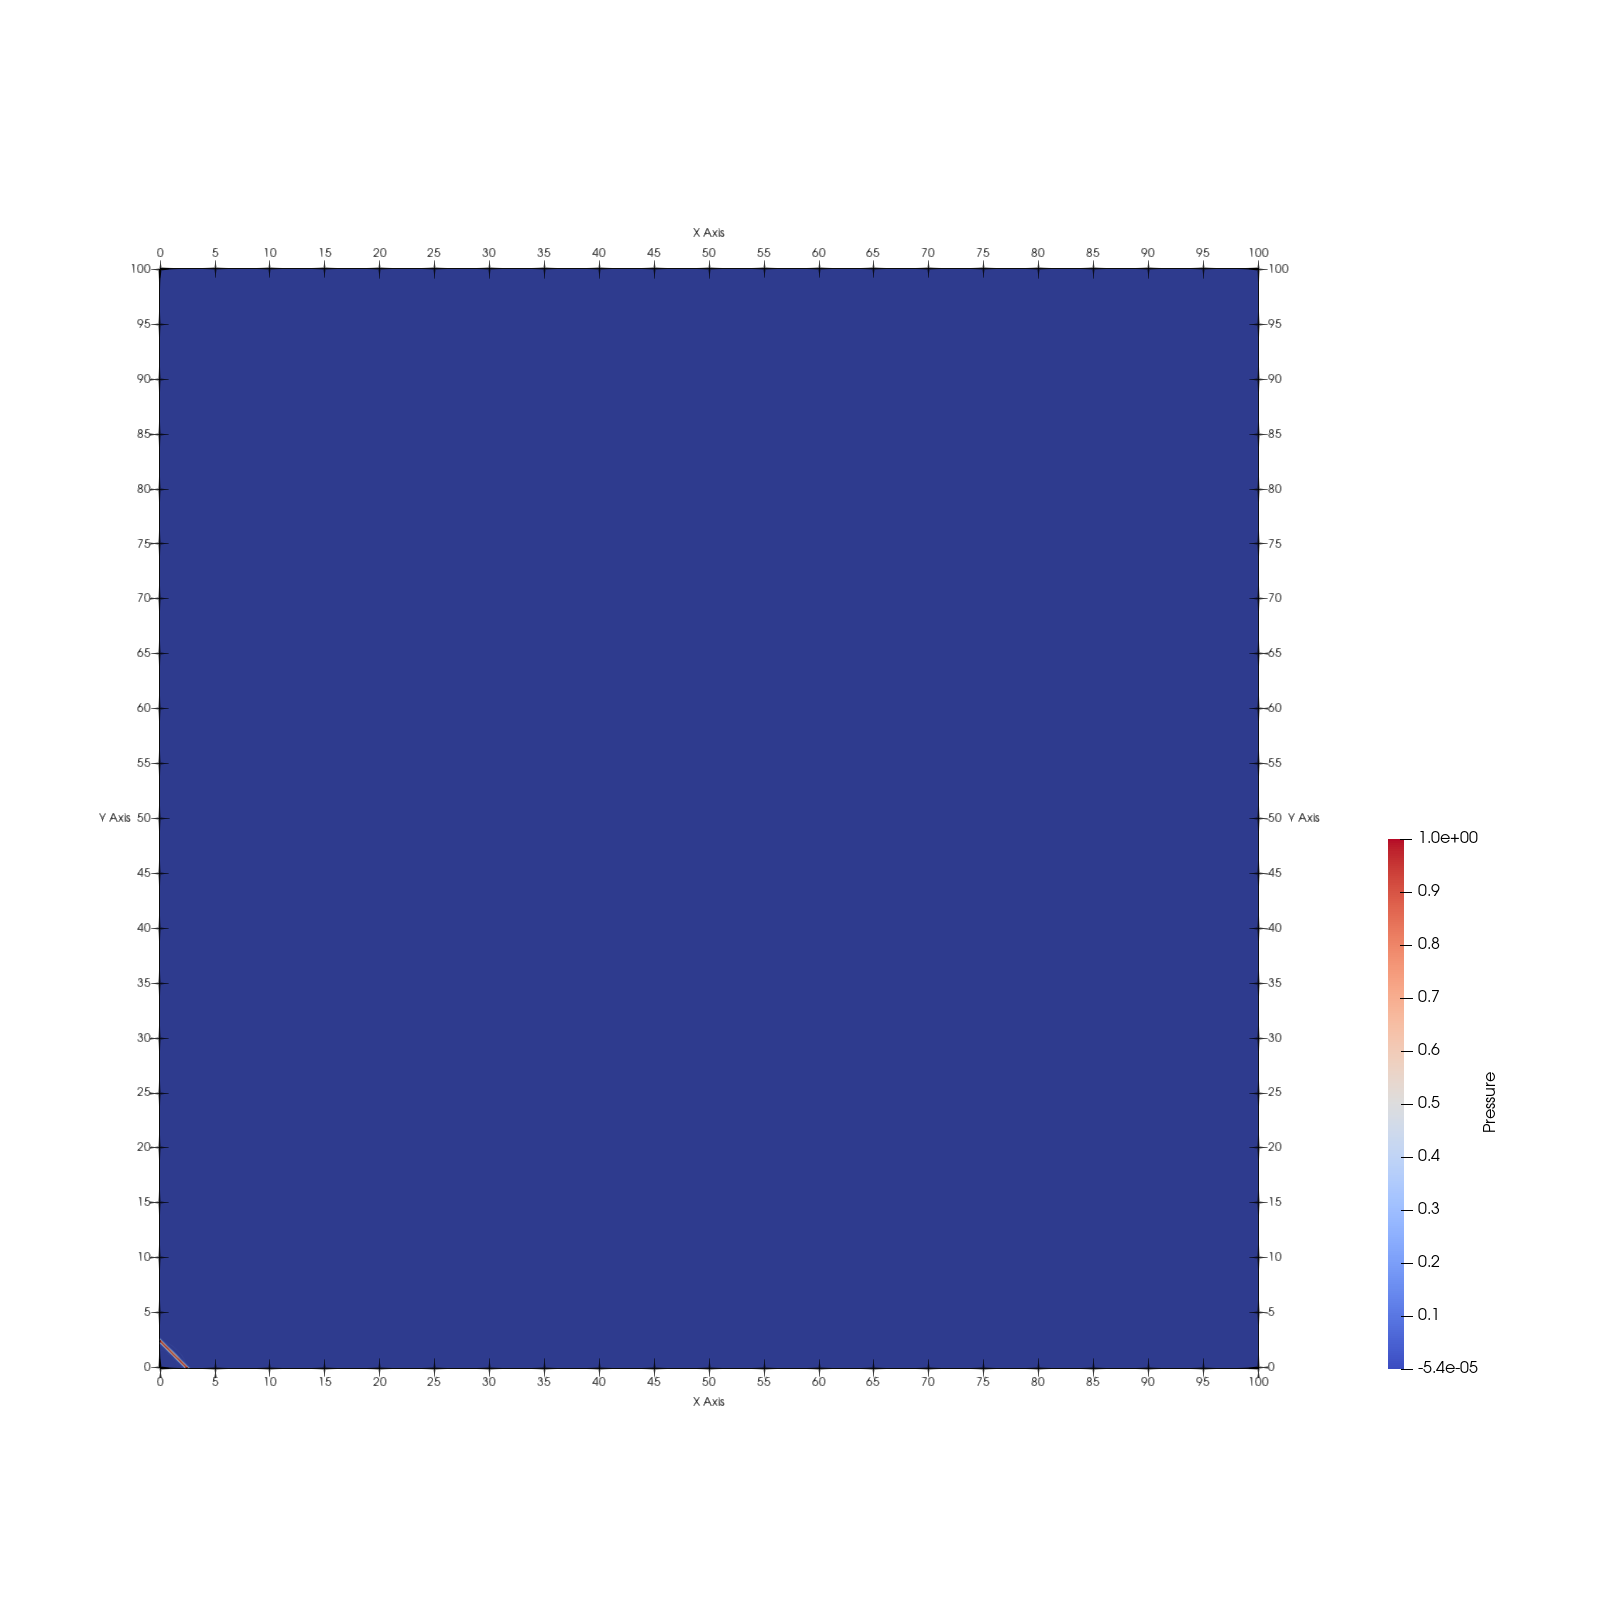
\includegraphics[width=0.45\textwidth]{Chapter_results/media/problem_big} \label{fig:load_imbalance_case_p}}
	\hfill
	\subfloat[Split level]
	{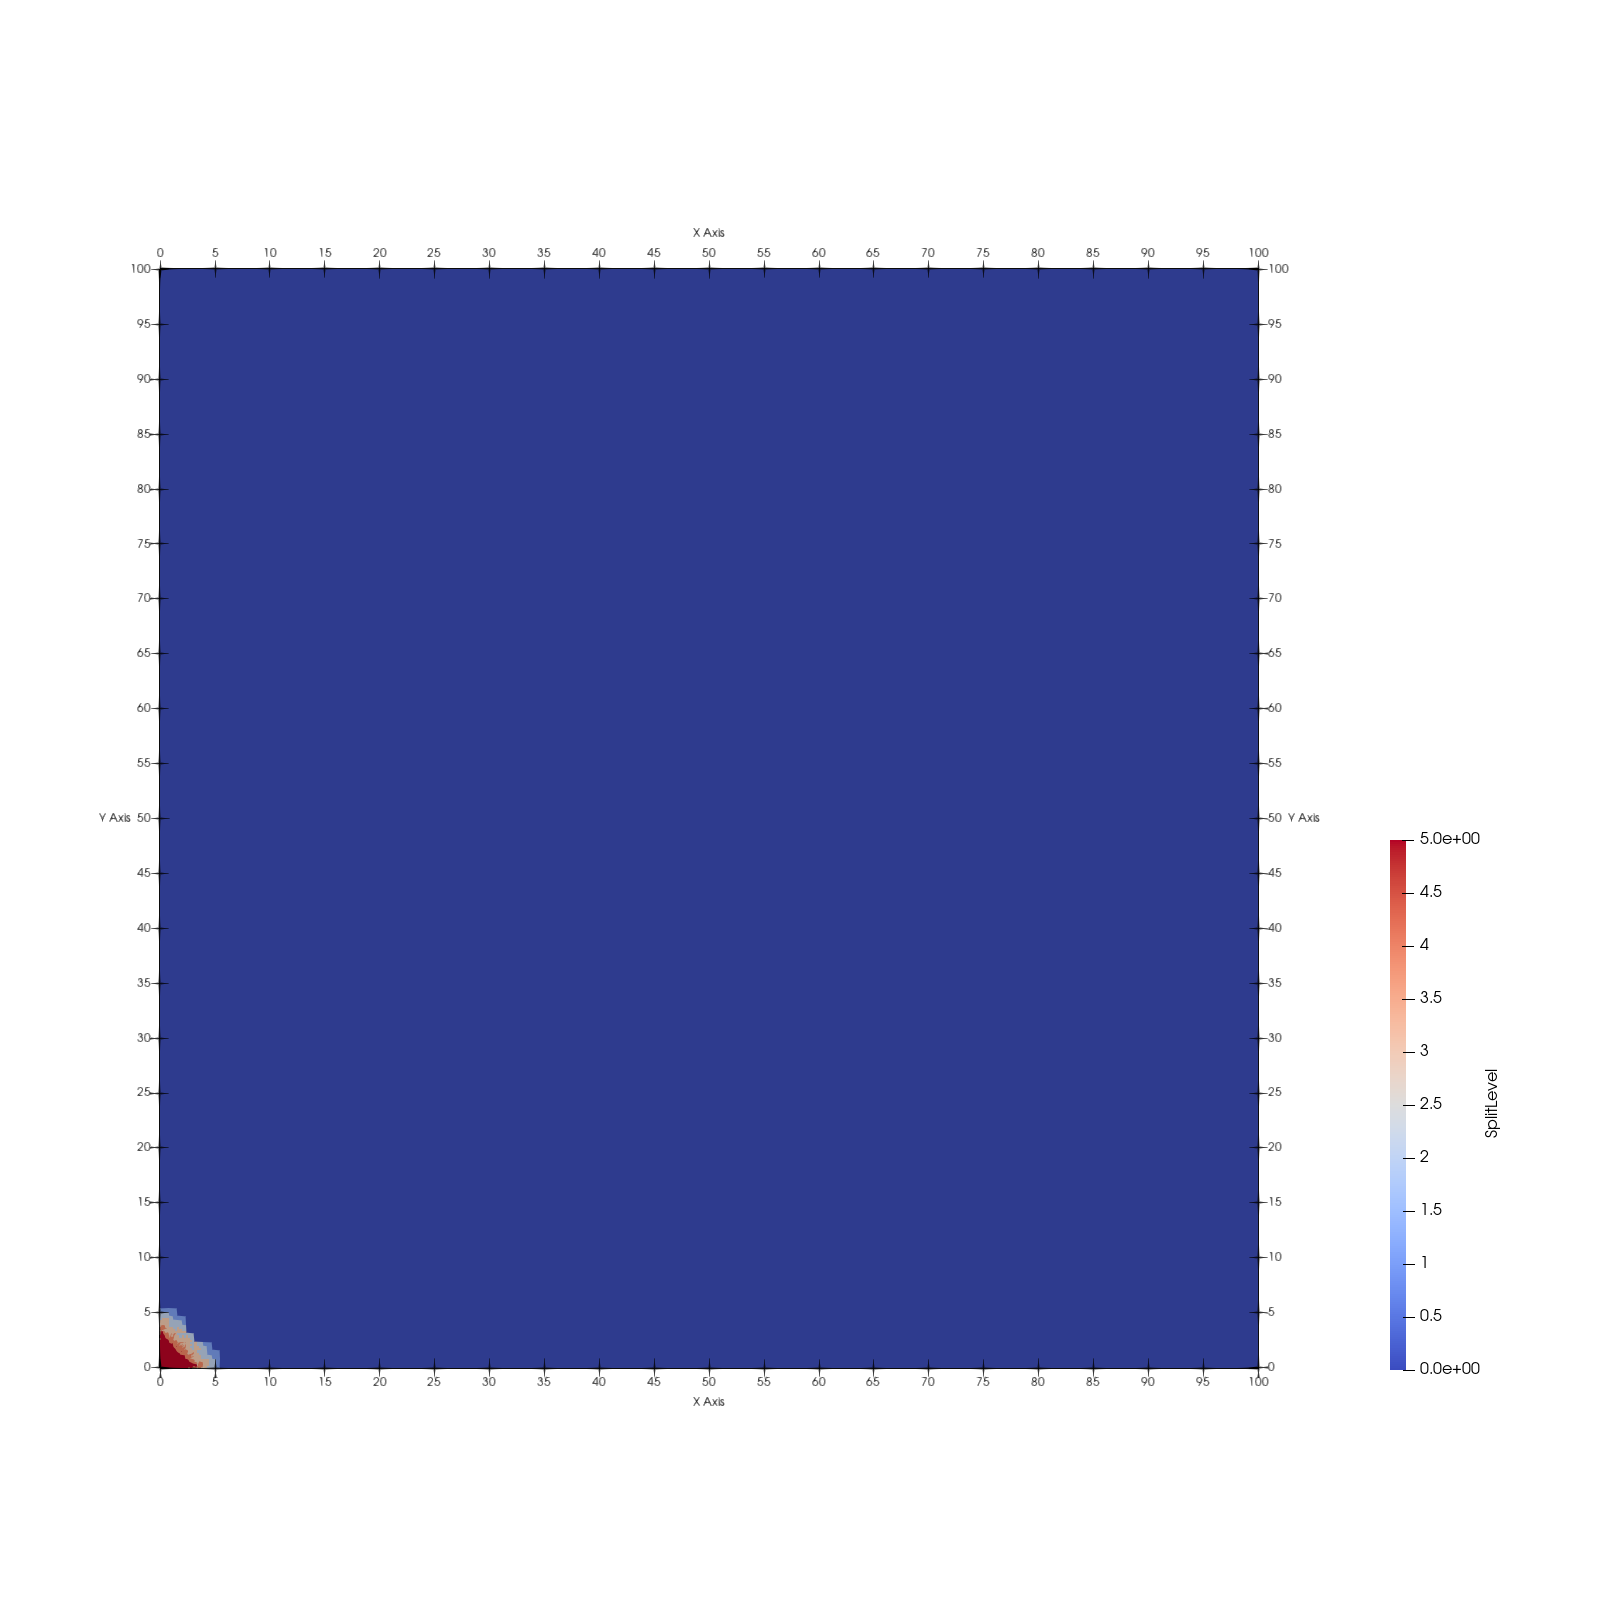
\includegraphics[width=0.45\textwidth]{Chapter_results/media/split_level_big} \label{fig:load_imbalance_case_s}}
	\caption{Load imbalance test case: A wave passes through a very big domain, only the bottom right refines. (a) Pressure (b) Split level, indicating how many times the elements have split}
	\label{fig:load_imbalance_case}
\end{figure}

% Table of imbalance

\subsection{Load balancing interval} \label{section:results:load_balancing_performance:interval}

\begin{figure}[H]
	\centering
	\includesvg[width=0.6\textwidth]{Chapter_results/media/load_balancing_interval_N4_K16384_A20_P16_S3}
	\caption{Load balancing efficiency interval test: Simulation time with adaptivity, load balancing and increasing load balancing interval. N = 4, K = 16384, adaptivity interval = 20, P = 16, max split level = 3}
	\label{fig:load_balancing_efficiency_interval}
\end{figure}

\subsection{Load balancing threshold} \label{section:results:load_balancing_performance:threshold}

\begin{figure}[H]
	\centering
	\includesvg[width=0.6\textwidth]{Chapter_results/media/load_balancing_threshold_N4_K16384_A20_L20_P16_S3}
	\caption{Load balancing efficiency threshold test: Simulation time with adaptivity, load balancing and increasing load balancing threshold. N = 4, K = 16384, adaptivity interval = 20, load balancing interval = 20, P = 16, max split level = 3}
	\label{fig:load_balancing_efficiency_threshold_s3}
\end{figure}

\begin{figure}[H]
	\centering
	\includesvg[width=0.6\textwidth]{Chapter_results/media/load_balancing_threshold_N4_K16384_A20_L20_P16_S5}
	\caption{Load balancing efficiency threshold test: Simulation time with adaptivity, load balancing and increasing load balancing threshold. N = 4, K = 16384, adaptivity interval = 20, load balancing interval = 20, P = 16, max split level = 3}
	\label{fig:load_balancing_efficiency_threshold_s5}
\end{figure}

\subsection{Polynomial order influence}
\label{section:results:load_balancing_performance:polynomial_order}

\begin{figure}[H]
	\centering
	\includesvg[width=0.6\textwidth]{Chapter_results/media/N_iteration_time}
	\caption{Polynomial order influence: Iteration time with increasing polynomial order.}
	\label{fig:N_influence}
\end{figure}

\section{Complex meshes} \label{section:results:complex_meshes}

\begin{figure}[H]
	\centering
	\subfloat[Circular domain]
	{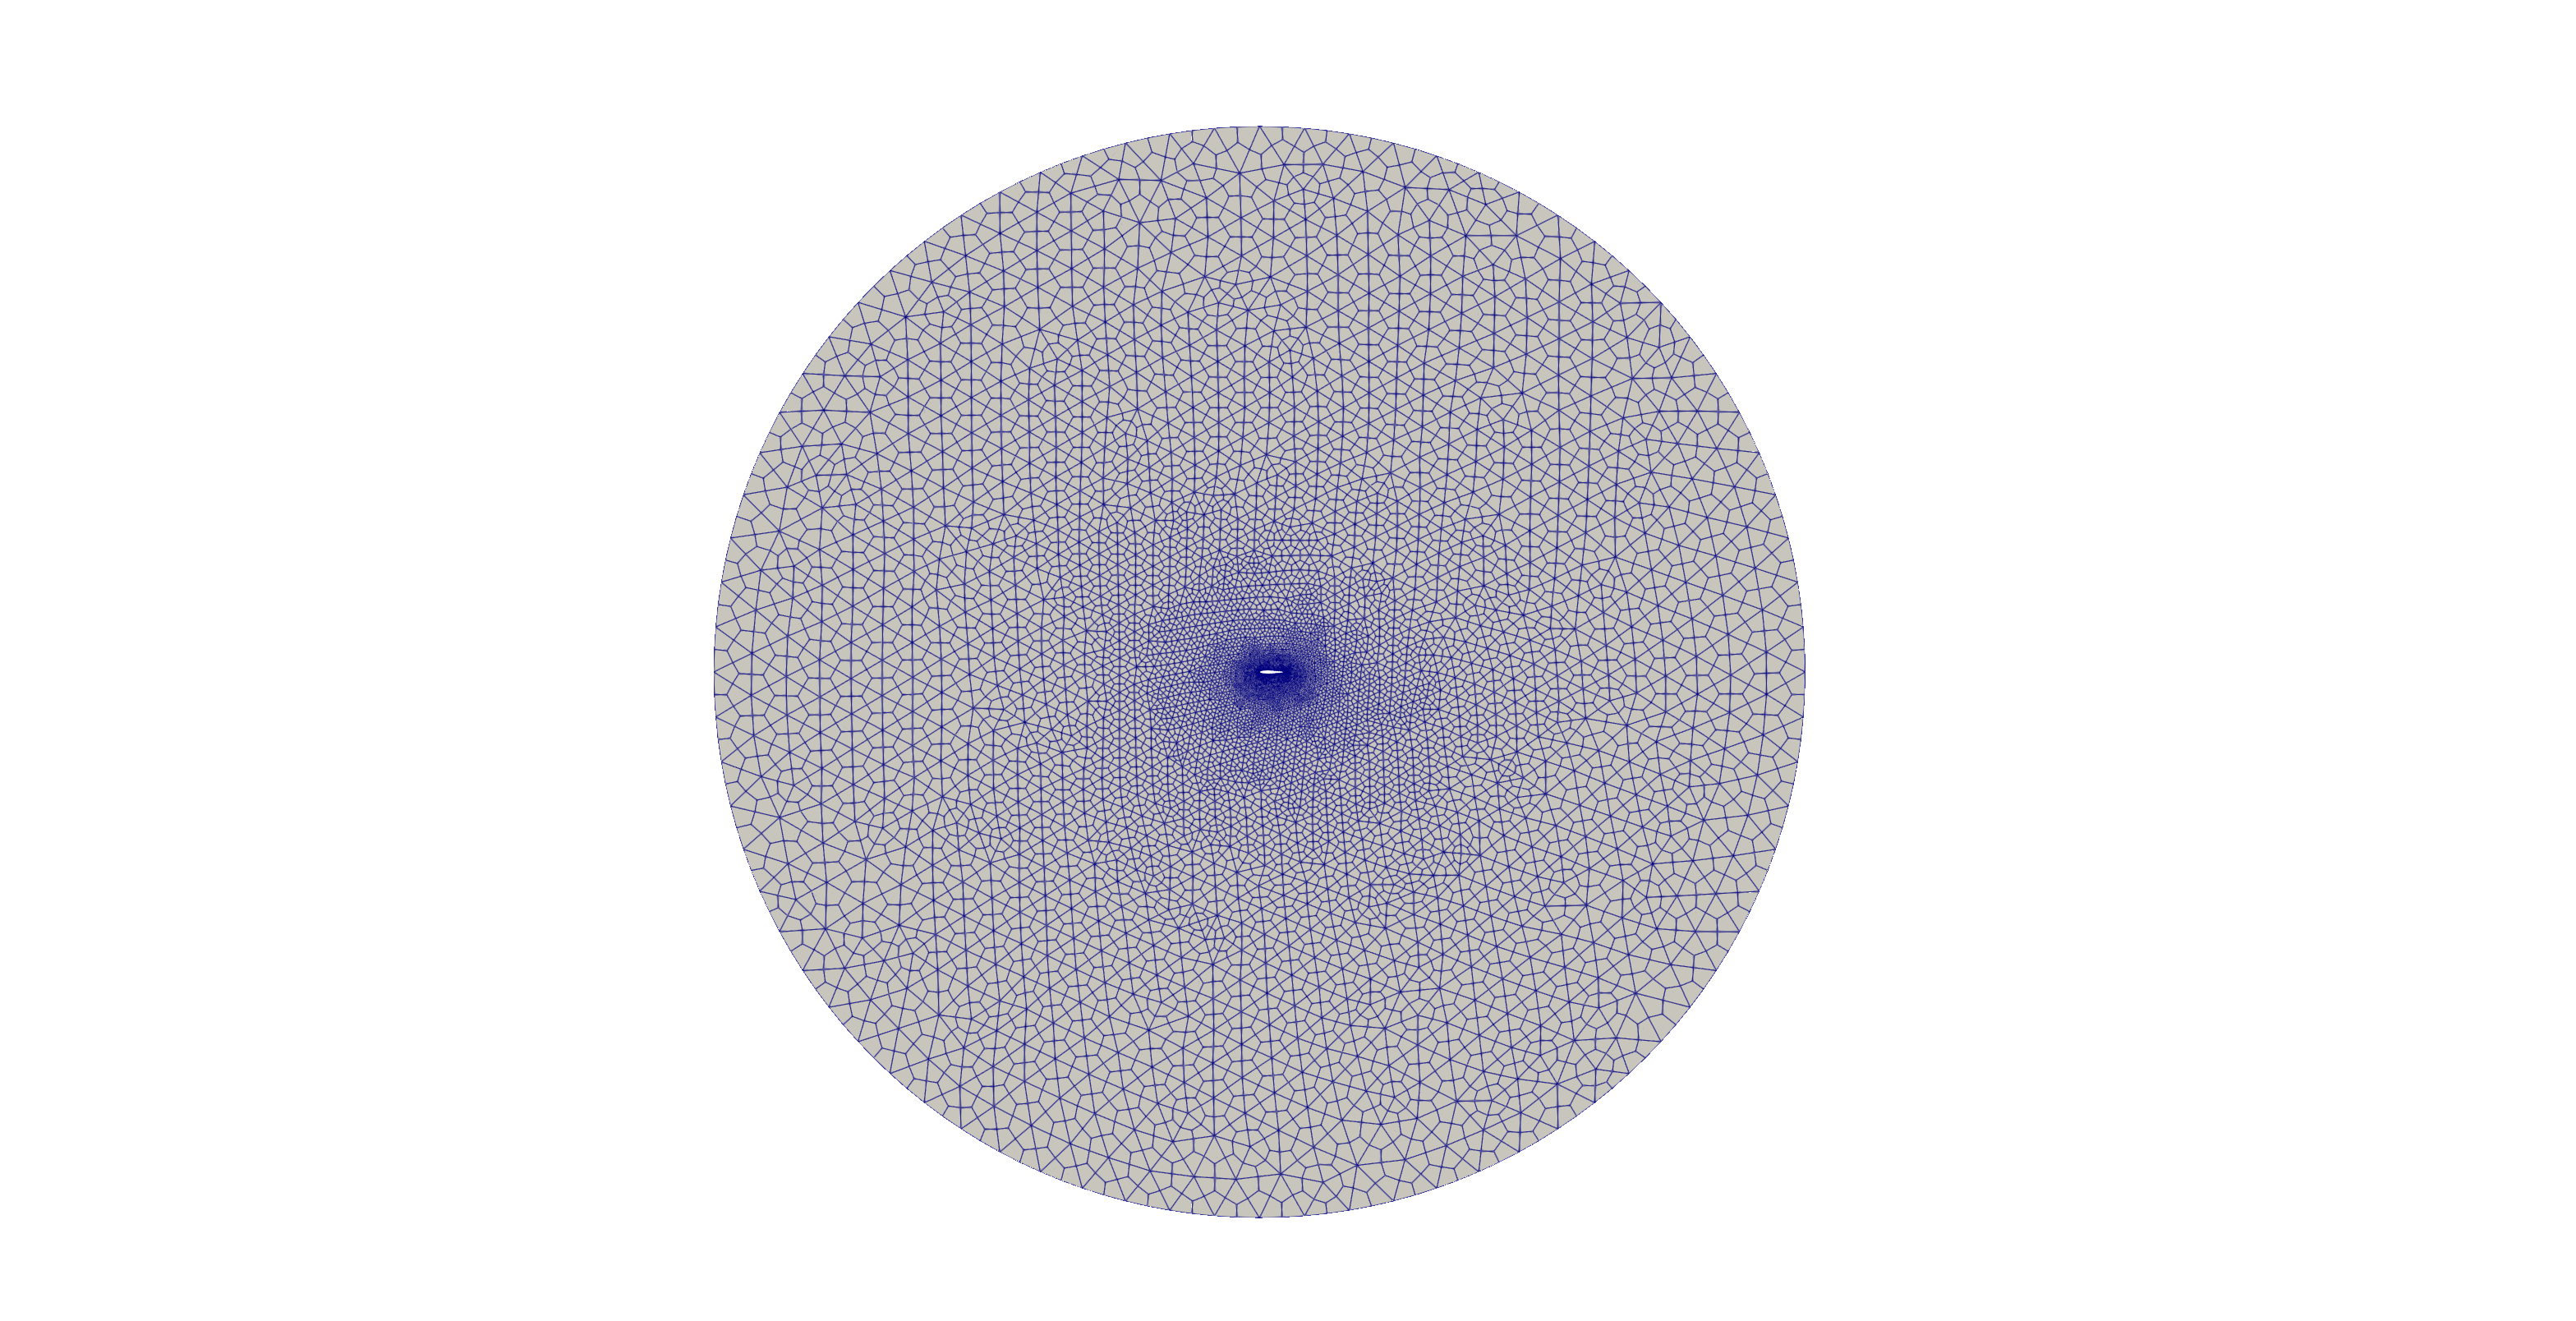
\includegraphics[width=0.45\textwidth]{Chapter_results/media/airfoil_mesh} \label{fig:complex_mesh_close}}
	\hfill
	\subfloat[Airfoil]
	{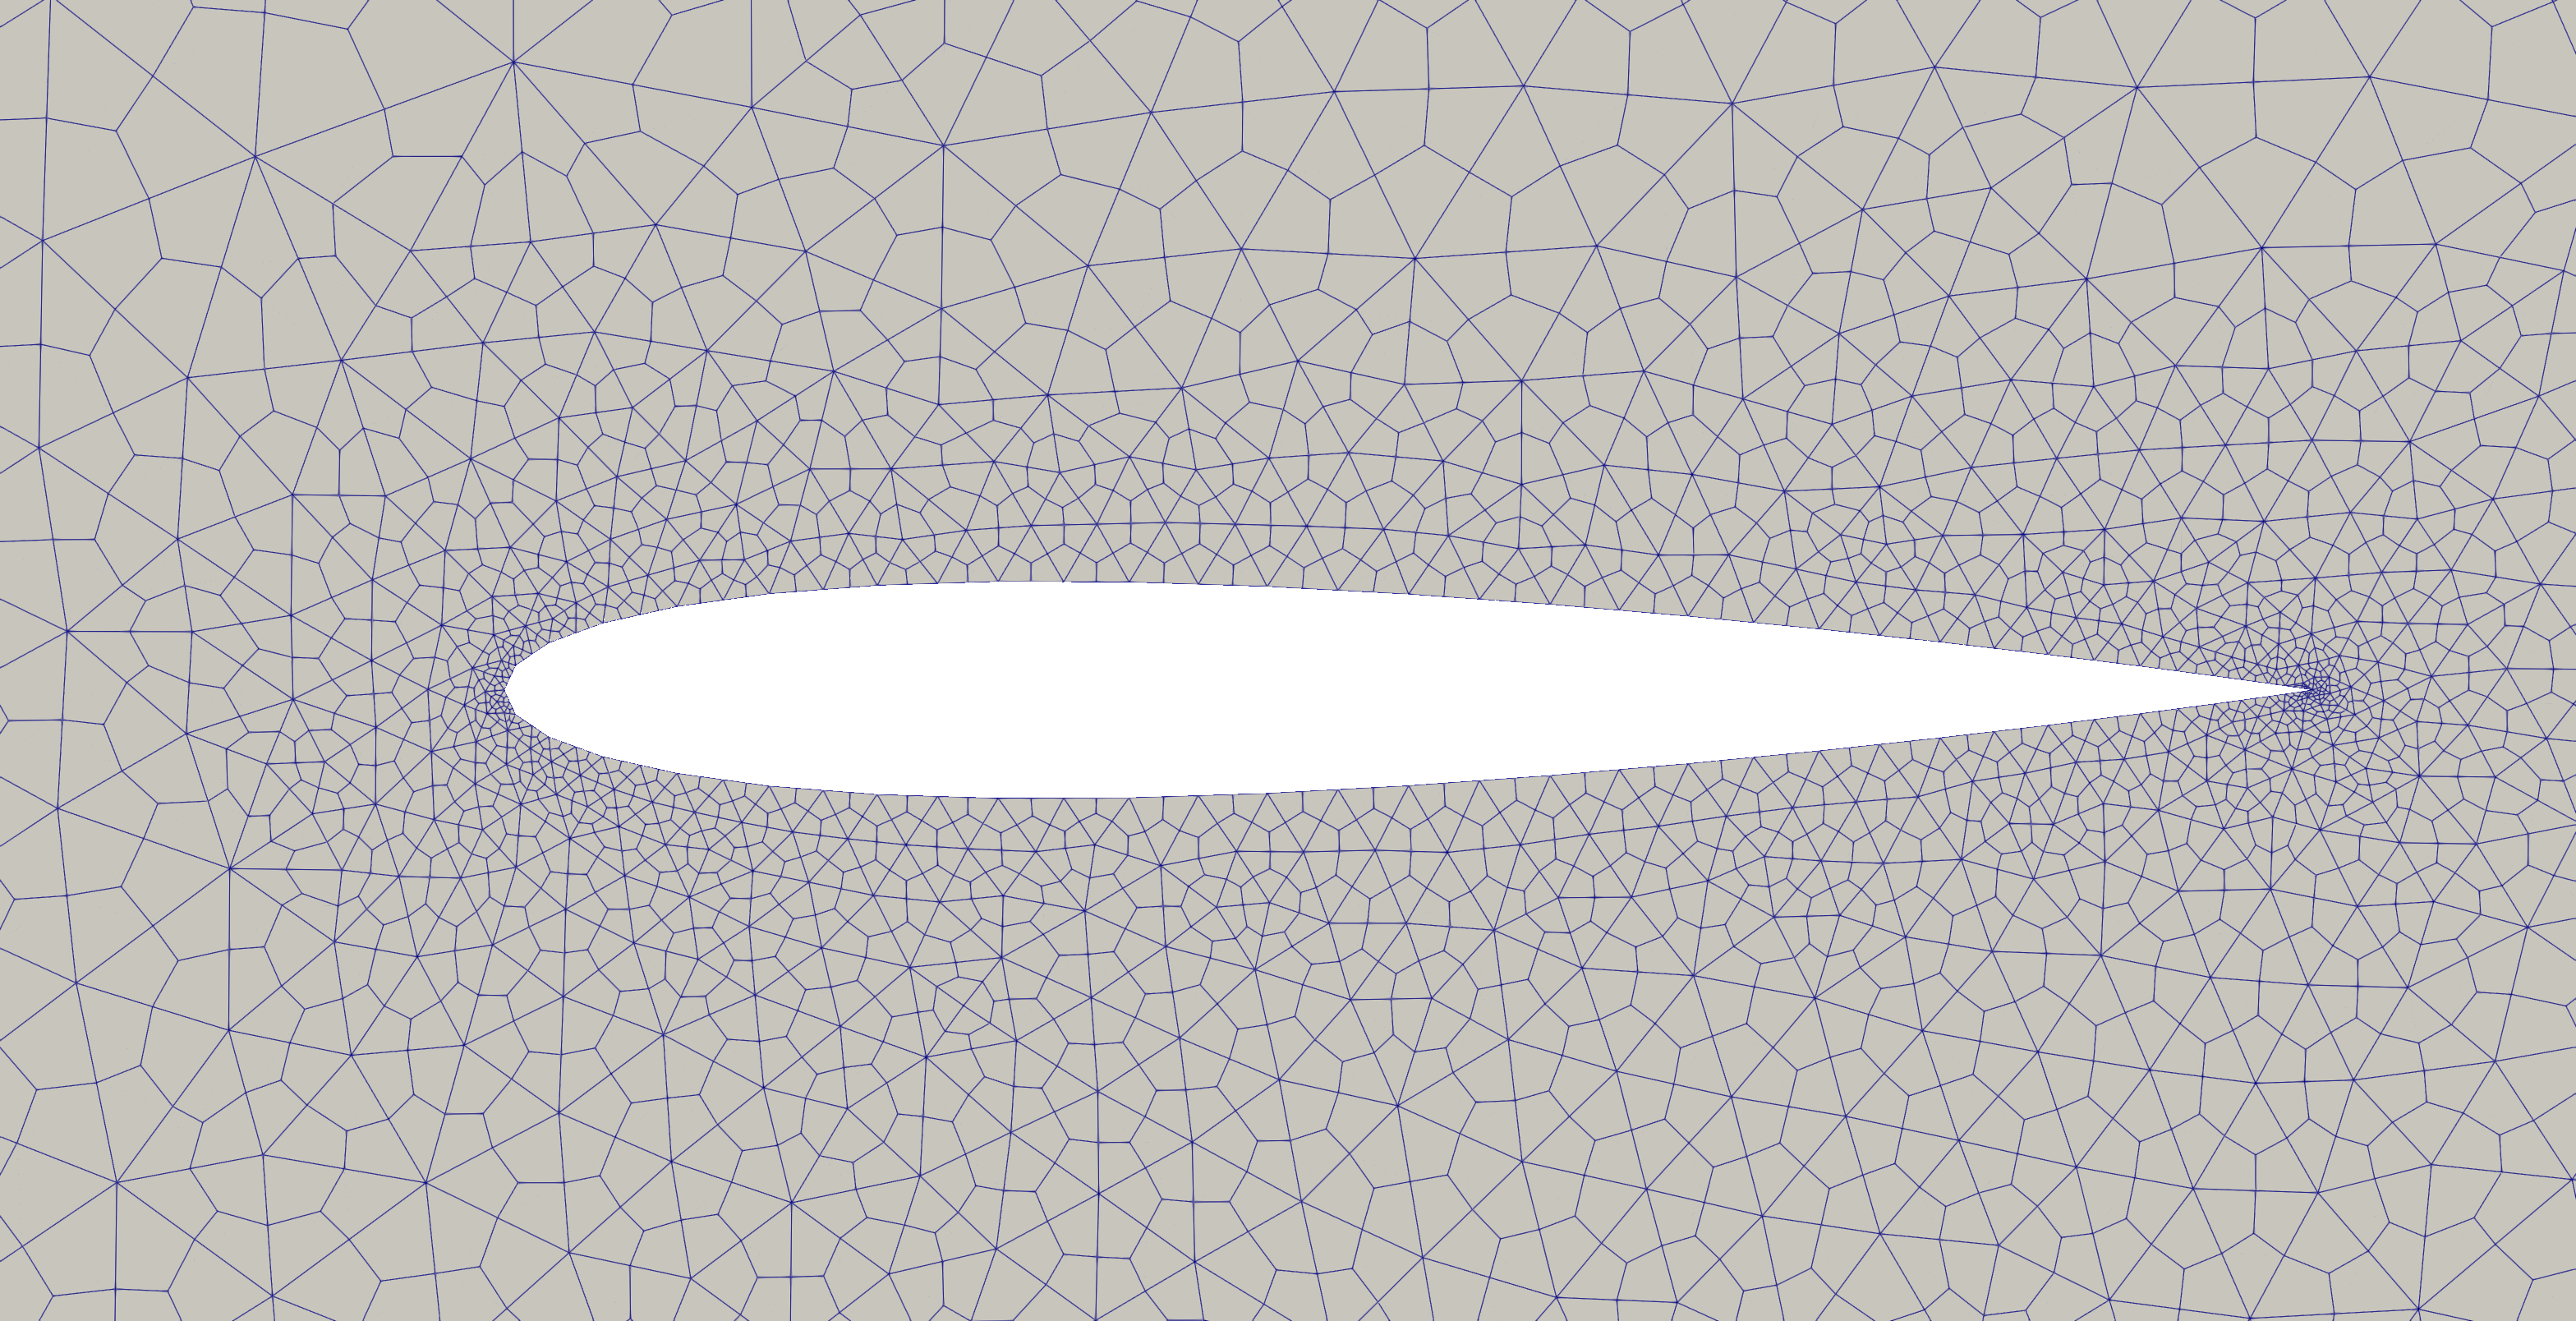
\includegraphics[width=0.45\textwidth]{Chapter_results/media/airfoil_mesh_close} \label{fig:complex_mesh_far}}
	\caption{Complex mesh: An airfoil in an unstructured circular domain. (a) Complete domain (b) Up close}
	\label{fig:complex_mesh}
\end{figure}

\begin{figure}[H]
	\centering
	\subfloat[Pressure]
	{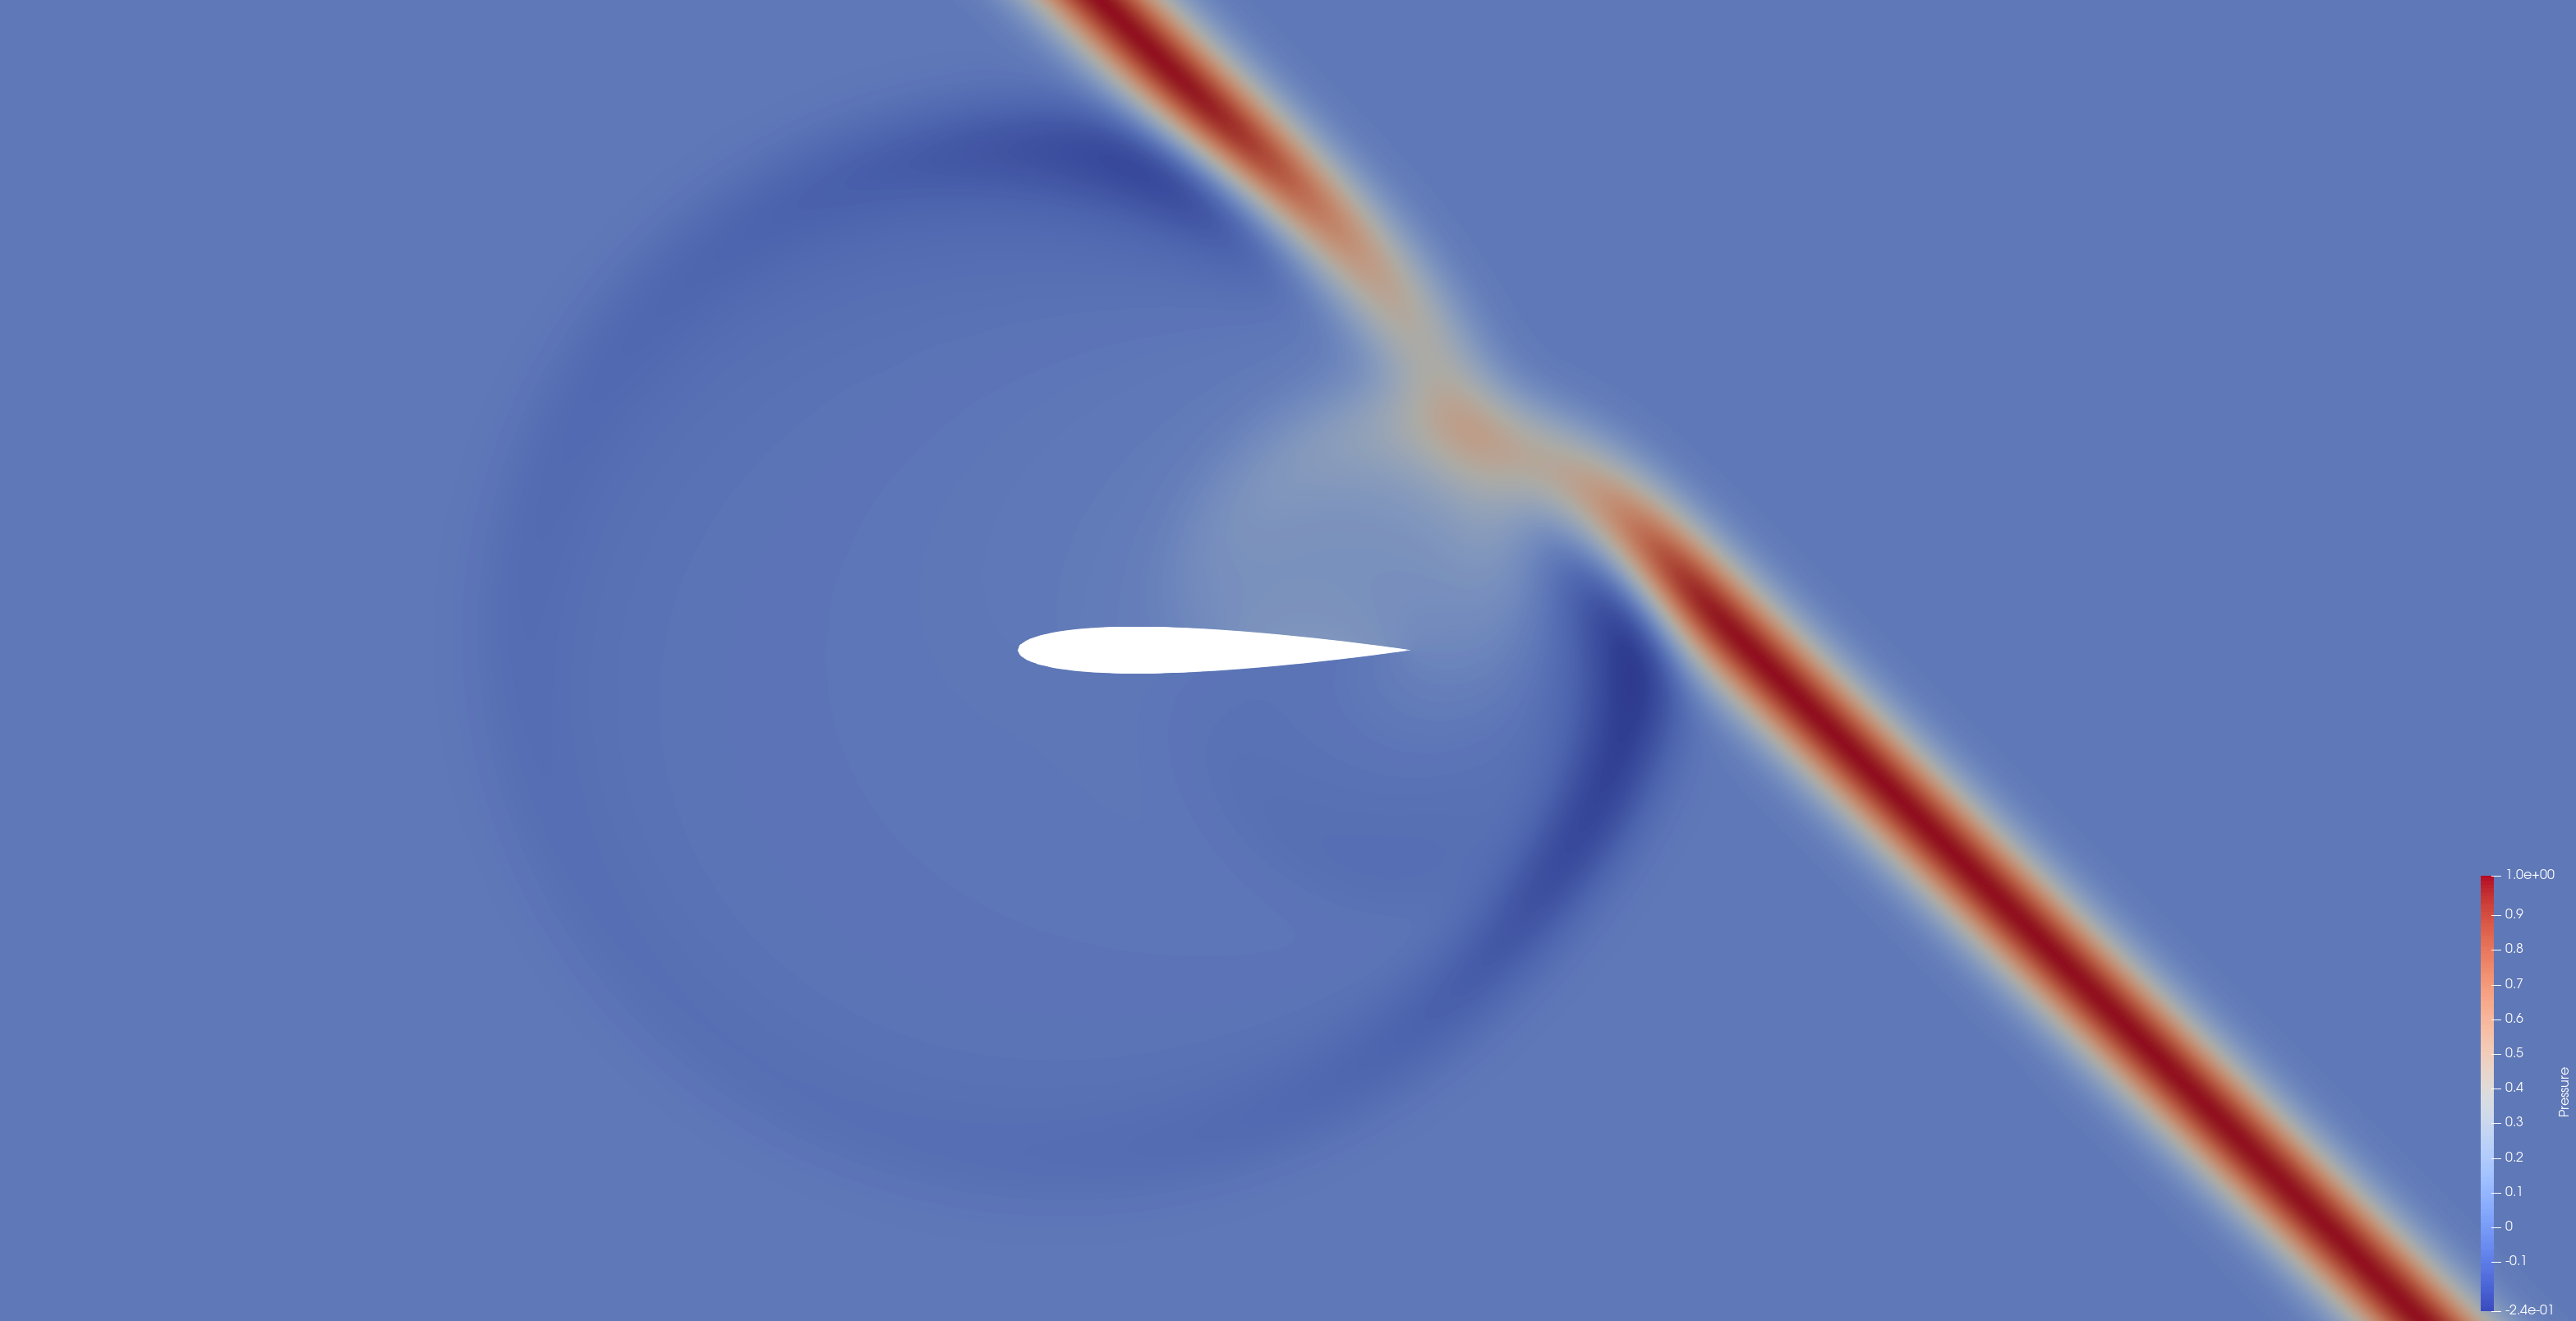
\includegraphics[width=0.45\textwidth]{Chapter_results/media/airfoil_pressure_close_t1_6} \label{fig:complex_mesh_solution_close}}
	\hfill
	\subfloat[Pressure $\sigma$]
	{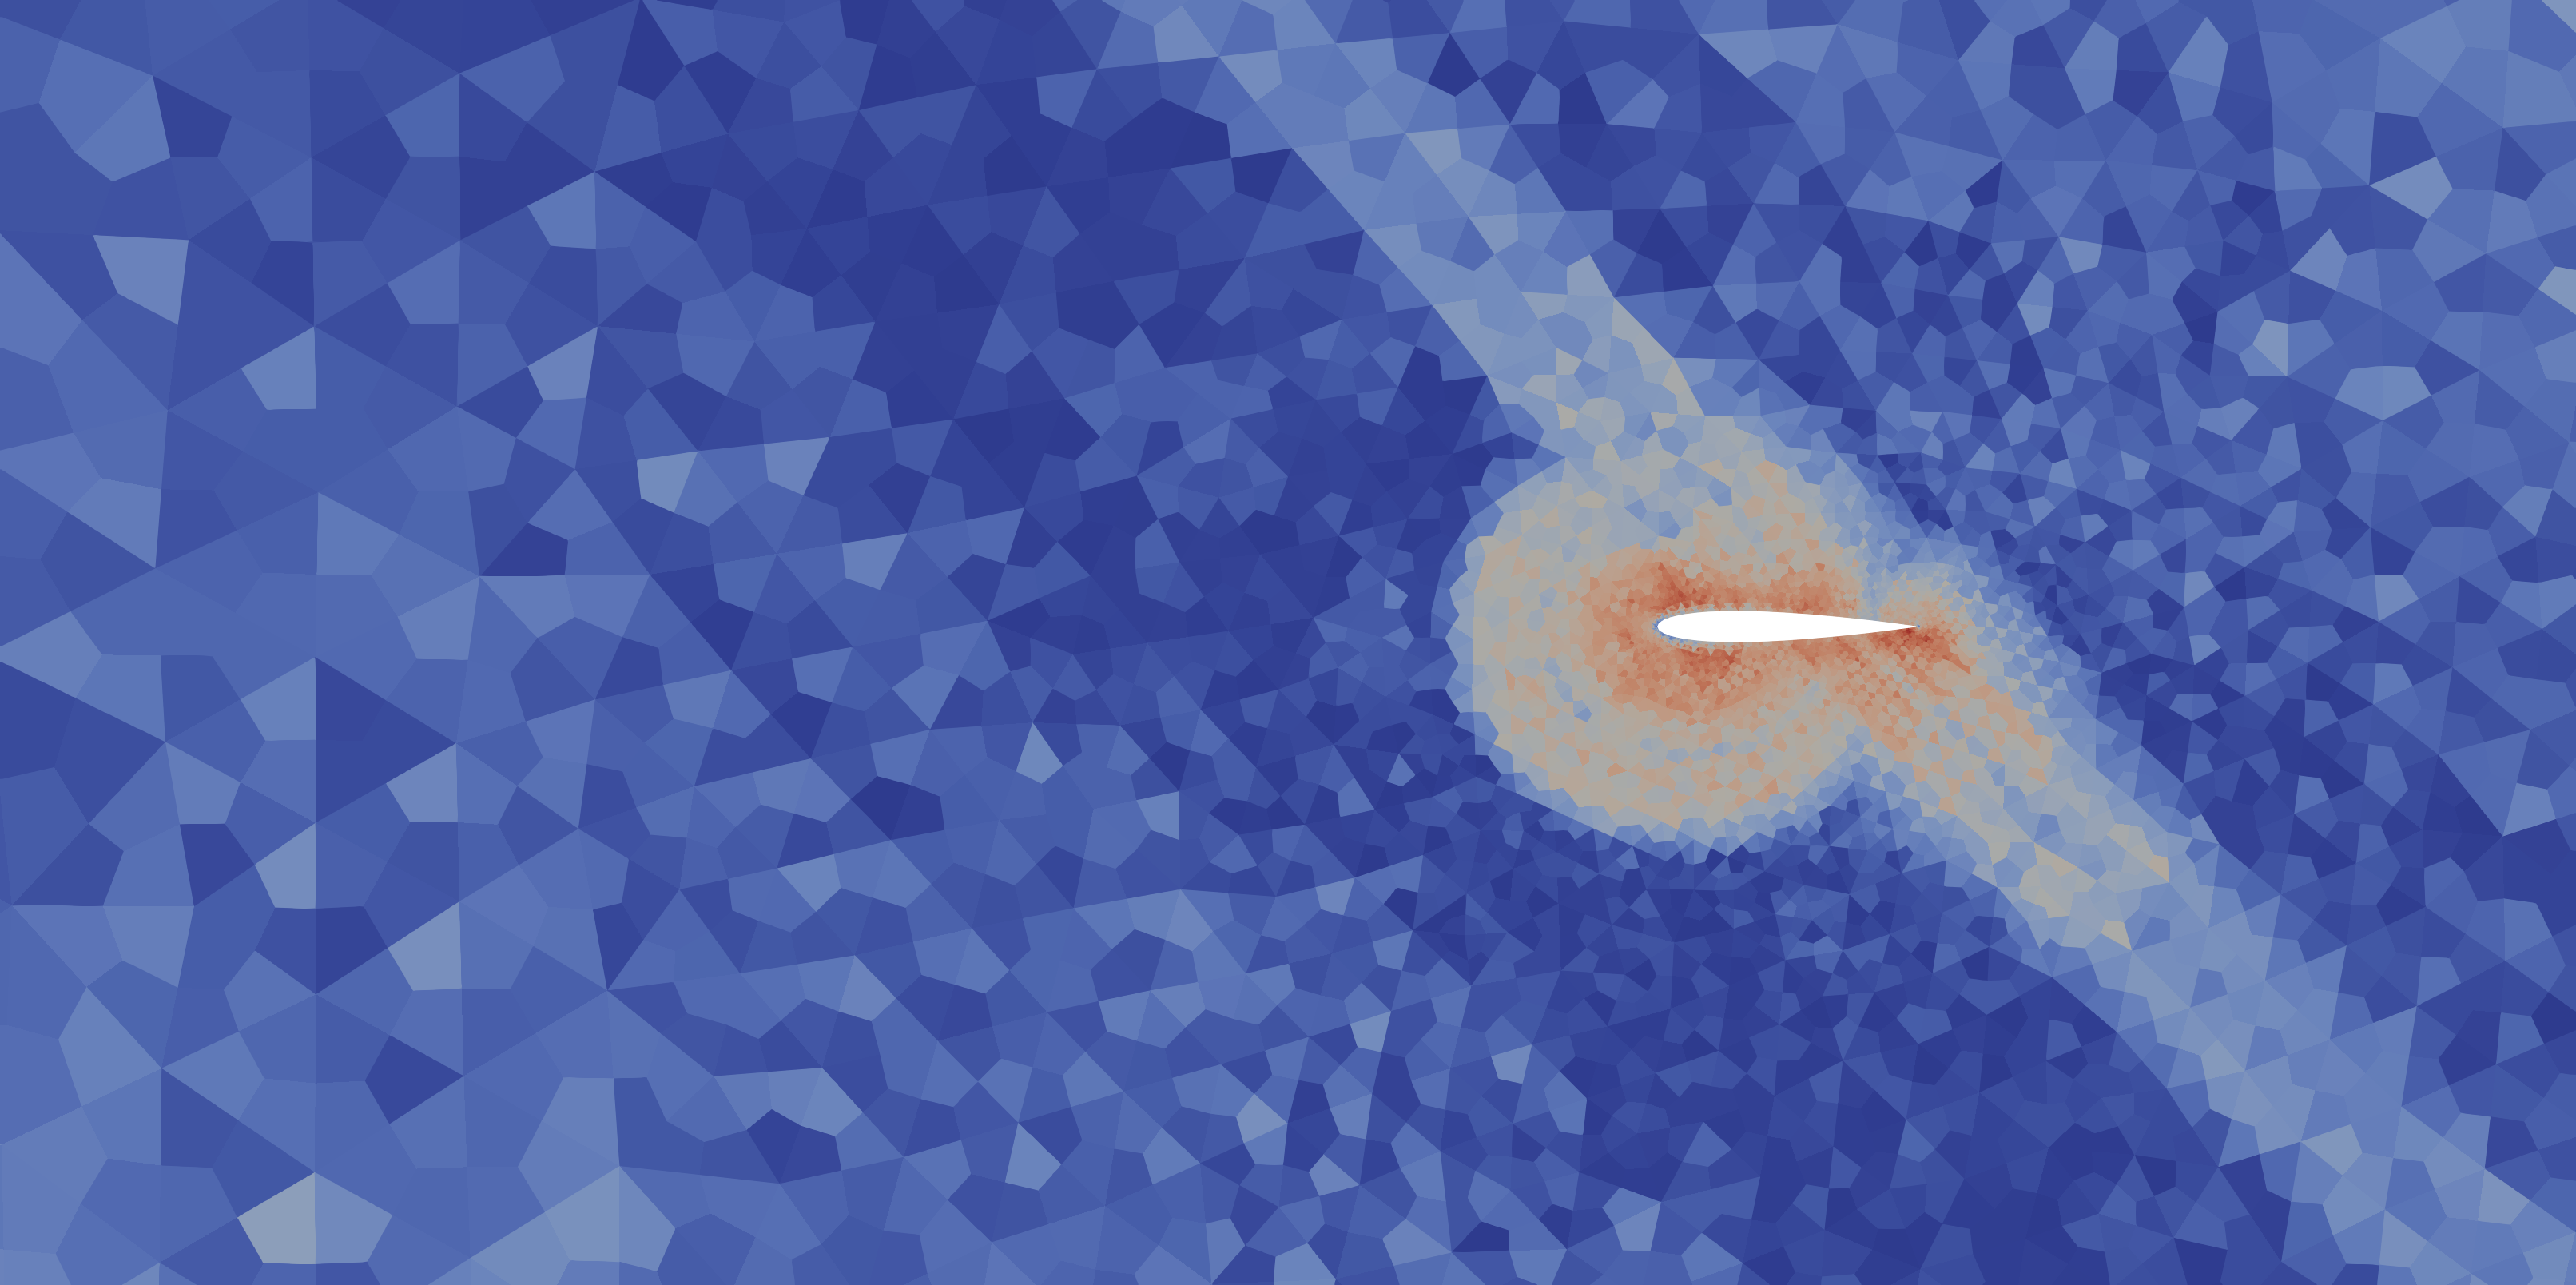
\includegraphics[width=0.45\textwidth]{Chapter_results/media/Airfoil 4} \label{fig:complex_mesh_solution_far}}
	\caption{Complex mesh: A wave going over an airfoil. (a) Pressure (b) Pressure $\sigma$, denoting if h-refinement or p-refinement would be chosen}
	\label{fig:complex_mesh_solution}
\end{figure}
